\chapter{Causal Inference Based Fault Localization for Numerical Software with Bayesian Additive Regression Trees}\label{chap:BART}


\section{Introduction}\label{BARTintro}
\vspace{-2pt}
With causal inference based SFL techniques\cite{bai2015numfl, baah2010causal, baah2011mitigating,shu2013mfl}, fault localization basically contains two steps: (1) controlling the confounding bias which is caused by confounding variables. (2) estimating the average failure causing effect of treatment variable $T$ on outcome $Y$. The second step, AFCE estimation, is a challenging because the functional form of the relationship between $T$ and $Y$ is unknown. The previous work, Baah et al’s used a parametric linear regression model to estimate a statement's AFCE. NUMFL used a quadratic regression model which a requires the user to pre-define the functional form of the dose-response function of the treatment $T$ (e.g. Figure 3.4). But if the parametric model is misspecified,, then AFCE estimation can be biased.

To solve the above problem in general settings, a non-parametric causal effect estimation model called Bayesian Additive Regression Trees(BART) has been proposed by Hill et al \cite{hill2012bayesian}. BART uses a sum-of-trees structure to approximate the dose-response function (DRF) of both the treatment variable and the confounding variables. 
Comparing to methods such as NUMFL and Baah et al’s causal estimator, BART requires less guess-work in modeling dose-response function.   

In this chapter, we proposal a new statistical fault localization method based on a BART model and evaluate it on numerical programs with single or multiple faults. The motivation for using BART in statistical fault localization is:
\vspace{-0.2cm}
\begin{itemize}
\item BART can flexibly fit non-linear response surfaces even with a large number of predictors
\item BART does not require the researcher to specify the functional form of the relationship between treatment and outcome. The user only needs to input the treatment, confounding variable and the outcome, but does not need to specify how these variables are parametrically related. Also, unlikely NUMFL, BART does not require a separate step to control confounding bias.
\item In an empirical study conducted by Hill et al., BART performed more effectively than propensity score matching based causal inference methods in average causal effect estimation for binary treatments. They also extended BART to detect the nonlinear relationship between continuous treatment and outcome. \cite{hill2012bayesian, hill2013assessing}.
\item Software is freely available and easy to use \cite{BARTMachine}.
\end{itemize}

The rest of the chapter is organized as follows: we present background on regression tree and BART model in Section \ref{BARTbg}; using BART to estimate the failure-causing effect of a program expression is described in detail in Section \ref{BARTafce};  we report on ourempirical evaluation of this approach in Section \ref{BARTevaluation}; related work is surveyed in Section \ref{BARTrelatedwork}; and Section \ref{BARTconclusion} concludes the chapter.

\section{BART Model Algorithm}\label{BARTbg}%what is BART and why BART
The BART model algorithm consists of three parts: a sum of trees model, a regularization prior and a fitting algorithm, Markov Chain Monte Carlo (MCMC)
\subsection{Single Regression Tree Model}
A regression tree is one type of decision tree that predicts the value of a target variable based on several input variables \cite{loh2011classification}, which handles the situation when the target variable is continuous. Figure \ref{singlergt} shows a single regression tree model. All the interior nodes of a regression tree have decision rules which send the input data set to either left or right side. After the input data set goes through the interior nodes and reaches the bottom of the tree, it is divided into several disjoint subgroups. Each group of data is represent by a leaf node.

\begin{figure*}[!thpb]
\centering
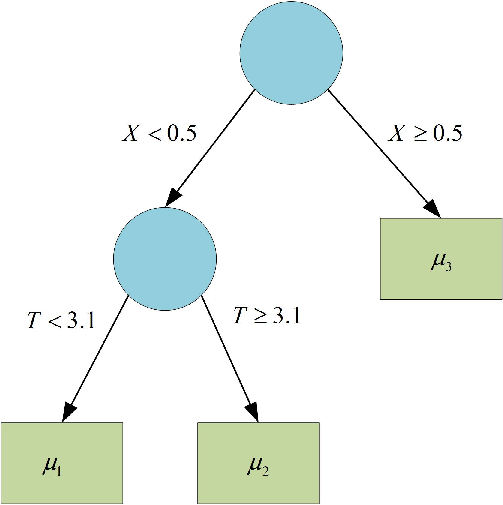
\includegraphics[width=0.5\textwidth]{chapter4_SingleRGT.pdf}
\caption{Single Regression Tree Structure}
\label{singlergt}
\end{figure*}

A single regression tree model is denoted as:
\begin{equation*}
Y=g(\pmb{Z}; R, M)+\epsilon
\end{equation*}
Here $\varepsilon  \sim N(0,{\sigma ^2})$ is a normally distributed error. $\pmb{Z}=[T,\pmb{X}]$ denotes all the variables related to the outcome $Y$, so $Z$ includes both treatment variable $T$ and confounding variables $\pmb{X}$. $R$ denotes a binary regression tree consisting a set of interior node decision rules and a set of terminal nodes, and $M=
{
 \mu _1, \mu _2, . . ., \mu _b
}$
denotes a set of parameter value associated with each of the $b$ terminal nodes of $R$. Each terminal node represent a regression model of outcome $Y$ on all the variables $Z$.

A regression tree model is often used in approximating unknown functions, such as, the dose-response function of the treatment variable, $Y=f(T,\pmb{X})$. The regression tree model divides the value space of $[T,\pmb{X}]$ in to several subgroups with its tree structure and a regression model is fitted for each subgroup. When making an inference about $Y$ given a specific unit of treatment and confounding variables values $[T=t,\pmb{X}=\pmb{x}]$, the regression tree will first find out which subgroup the unit belongs to and then infer outcome $Y$ with the corresponding linear regression. A regression tree model has two advantages: (1) making prediction is fast (2) it can handle non-linear function approximation.  The limitation of regression tree model is that a regression tree model may be an unstable decision tree. In other words, insignificant modification of learning sample, such as eliminating several observations, could lead to radical changes in the tree structure: increase or decrease of tree complexity, changes in splitting variables and values \cite{timofeev2004classification}.


\subsection{A sum-of-trees model}
BART is a sum-of-trees model. With the definition of a single tree model, the sum-of-trees model can be expressed as:
\begin{equation*}
Y = g(\pmb{Z};{R_1},{M_1}) + g(\pmb{Z};{R_1},{M_1}) +  \cdots  + g(\pmb{Z};{R_m},{M_m}) + \varepsilon
\end{equation*}
where each $(R_i,M_i)$ denotes a single sub-tree model and $\varepsilon  \sim N(0,{\sigma ^2})$.  $m$ denotes the number of trees in BART model. We have
 \begin{equation*}
 Y =f(\pmb{Z})=f(T,\pmb{X})= \left( {\sum\limits_{j = 1}^m {g(T,\pmb{X};{R_j},{M_j})} } \right) + \varepsilon
 \end{equation*}

Compared to single regression tree model, BART model has two advantages. First BART can incorporate interaction effects of varying orders. Unlike the single tree model, when $m>1$ the terminal node $\mu_i$ given by $g(\pmb{Z};{R_i},{M_i})$ is merely part of the conditional mean of $Y$ given $Z$. If the assignment of $\mu_i$ depends on just a single component of $Z$ (only one variable),  $\mu_i$  represents direct effect of that variable to $Y$. If the assignment of $\mu_i$ depends on more than one component of $Z$ (e.g., more than one variable), the terminal node will represent interaction effects of those variables. Because the BART model may be based on trees of varying sizes, the sum-of-trees structure can incorporate both direct effects and interaction effects of varying orders \cite{conference1997advances}. Second, fitting a BART model does not entail much more computation cost than fitting a large single tree model. This is because that BART can scale to large datasets using a parallel MCMC sampler \cite{pratola2014parallel, pratola2015bayesian}.  

\subsection{A regularization prior}
Fitting the BART model requires a prior distribution of all the parameters of the sum-of-trees model.  The prior regularizes the fit by keeping the individual tree's effect from being unduly influential. Without such a prior, large tree components would dominate the structure. The regularization prior can also help BART avoid overfitting. To simplify the prior specification, the trees in the BART model $(R_1, M_1), (R_2,M_2), \ldots, (R_m, M_m) $ are considered to be independent of each other and of $\sigma$. Also, the terminal node parameters $ \mu _{1j}, \mu _{2j}, . . ., \mu _{bj} $ of every tree $R_j$ are assumed to be independent. So we have:

\begin{equation*}
 \begin{array}{l}
P(({R_1},{M_1}),({R_2},{M_2}) \ldots ,({R_m},{M_m}),\sigma ) = \left[ {\prod\limits_j {P({R_j},{M_j})} } \right]p(\sigma )\\
\quad \quad \quad \quad \quad \quad \quad \quad \quad \quad \quad \quad \quad \quad \; = \left[ {\prod\limits_j {P({M_j}|{R_j})P({R_j})} } \right]p(\sigma )
\end{array}
 \end{equation*}
and
\begin{equation*}
P({M_j}|{R_j}) = \left[ {\prod\limits_i {P({\mu _{ij}}|{R_j})} } \right]
 \end{equation*}
Here ${\mu _{ij}} \in {M_j}$ denotes the $ith$ terminal node of the $jth$ regression tree. From the above equations, we can see that independence simplifies the problem of specifying the complete prior distribution to the specification of priors for just ${P({\mu _{ij}}|{R_j})}$, $P({R_j})$ and $P(\sigma)$. In \cite{chipman2010bart}, the specification of prior forms on $P(\sigma)$ is assumed to be an inverse chi-square distribution. The prior on ${P({\mu _{ij}}|{R_j})}$ is assumed to be a conjugate normal distribution. The prior on $P(R_j)$ is complex. It contains 3 aspects:
\begin{enumerate}
\item the probability that a node at depth $d$ is nonterminal, given by
\begin{equation*}
\alpha {(1 + d)^{ - \beta }},\quad \alpha  \in (0,1),\beta  \in [0,\infty )
 \end{equation*}
\item the prior probability that a variable is selected as the splitting variable at an interior node is $1/k$ and $k$ is the total number of variables including both treatment and confounders.
\item the prior probability that a splitting variable splitted at a specific value $x$ is $1/N$, and $N$ is the total number of observed values of the splitting variable in the sample data set.
\end{enumerate}
The details of the prior specification for ${P({\mu _{ij}}|{R_j})}$, $P({R_j})$ and $P(\sigma)$ can be found in reference \cite{chipman2010bart}.


\subsection{Bayesian Backfitting MCMC Algorithm}
BART uses an iterative Bayesian backfitting  MCMC algorithm to fit the model \cite{gilks2005markov}. The algorithm uses Gibbs sampler \cite{casella1992explaining}. The Gibbs sampler makes $m$ successive draws of $(R_j, M_j)$ conditionally on $(R_{(j)}, M_{(j)}, \sigma)$:

\begin{equation*}
(R_j,M_j)|R_{(j)}, M_{(j)}, \sigma, Y
\end{equation*}
$j=1 \ldots m$, followed by a draw of $\sigma$ from the full conditional:

\begin{equation*}
\sigma |{R_1}, \ldots ,{R_m},{M_1}, \ldots ,{M_m},Y
\end{equation*}
Here $R_{(j)}$ represents all the trees except $R_j$, so $R_{(j)}$ will be a set of $m-1$ trees. $M_{(j)}$ is similarly defined as $R_{(j)}$.

\section{AFCE Estimation With BART}\label{BARTafce}% how to use BART

In this section, we introduce our approach to using BART to estimate the AFCE of a numerical program expression, which is adapted from Hill et al. \cite{hill2012bayesian}. Hill et al. have proved that BART is effective in average causal effect estimation when the treatment variable is binary. In \cite{hill2012bayesian}, the causal effect of a binary treatment variable $T$ for individual $i$ is defined as $Y_i(1)-Y_i(0)$. $Y_i(1)$ and $Y_i(0)$ are the {\it potential outcomes} for individual $i$, which means the outcomes that would be observed under $T=0$ and $T=1$. Since $Y_i(1)$ and $Y_i(0)$ cannot be both observed fro any individual in the observational study, the causal effect is measured by the average causal effect $E[Y(1)-Y(0)]$.  Based on the potential outcome notation, we briefly reviewed Hill’s algorithm:

Hill et al. use BART to estimate average causal effects such as $E(Y(1)|\pmb{X}=\pmb{x}) - E(Y(0)|\pmb{X}=\pmb{x})=E(Y|T=1, \pmb{X}=\pmb{x})-E(Y|T=0, \pmb{X}=\pmb{x})=f(1,\pmb{x})-f(0,\pmb{x})$ . $f(t,\pmb{x})$ is the function that predicts the outcome $Y$ using the values of both treatment variable and confounding variables.  The algorithm contains the following steps:
\begin{enumerate}
\item Fit a BART model with the MCMC algorithm to the full sample.
\item Generate a posterior prediction for each unit by setting the treatment variable value to $T=1$ and keep the confounding variable values unchanged.
\item Generate a posterior prediction for each unit by setting the treatment variable value to $T=0$ and keep the confounding variable values unchanged.
\item Calculate the difference between the posterior predictions for each unit.
\item Estimate the average causal effect by averaging all the differences of posterior predictions.
\end{enumerate}

In step 1, the fitted BART model characterizes the causal relationship between treatment $T$ and outcome $Y$ given the confounders $\pmb{X}$. We can use the fitted model to predict the outcome $Y$ under different $(T, \pmb{X})$ conditions. For an untreated unit $(T=0, \pmb{X}=\pmb{x})$,  if we set the treatment variable to 1 and then input $(T=1, \pmb{X}=\pmb{x})$ into the BART model, the output is the estimated potential outcome $Y(1)$ for that unit in treated condition. Similarly, we can estimate the potential outcome $Y(0)$ of a treated unit in untreated condition by inputing $(T=0, \pmb{X}=\pmb{x})$ into the BART model. Thus, in steps 2 and 3, BART is used to predict the missing potential outcomes (counterfactual outcomes). Thus, the difference calculated in step 4 is the individual (unit) level causal effect. The average of these differences is average causal effect, which is estimated in step 5.

If the treatment variable is continuous,  we can use BART to approximate a function $Y=f(T,\pmb{X})$ that specifies the dose-response function of the continuous treatment $T$ and confounding variables $\pmb{X}$.  As we mentioned before, BART model does not require the user to make assumptions or specify the functional form of the dose-response function.  But AFCE estimation for numerical expressions with BART is challenging. In previous CSFL methods (e.g. NUMFL or Baah et al’s causal estimator), the average failure-causing effect can be characterized by the coefficient of a regression model.  But with the BART model, each tree $g(\pmb{Z};{R_1},{M_1})$ only explains part of $Y$, so there are no parameters in BART that can directly characterize the AFCE. 

To solve this problem, we proposed a novel BART based average causal effect estimation algorithm for continuous treatment. We first estimate the individual-level causal effect for  each unit in the sample. Then the average value of the estimated individual-level causal effects in the data set is the estimated AFCE of the expression.  Assume the unit $i$ has treatment variable $T=t$ and confounding variables $\pmb {X}=\pmb {x}$, we can use the fitted BART model to estimate the outcome for the unit $y=f(t,\pmb{x})$. Then we increase the treatment variable to $t'=t+\varepsilon$, here $\varepsilon $ is a small number. We input $t'$ and $\pmb{x}$ into the fitted BART model and get the estimated posterior $y'=f(t',\pmb{x})$. Then the estimated causal effect of $T$ on $Y$ for unit $i$ is $\left| {y - y'} \right|$. The algorithm is as follows:
\begin{enumerate}
\item Fit a BART model using MCMC algorithm to the full sample.
\item Given a unit in the observational data set, we input it into the fitted BART model. 
\item increase the value of the treatment variable from $t$ to $t'=t+\varepsilon$, but keep the confounding variables unchanged. The causal effect of treatment for this unit is estimated by the change in the output of the BART model $|f(t',\pmb{x})-f(t,\pmb{x})|$.
\item repeat step 2 and step 3 for all the unit in the dataset.
\item Estimate failure-causing effect by averaging all the differences of posterior predictions.
\end{enumerate}

In the above algorithm, the BART model fitted in step 1 is used to approximate DRF $Y=f(T,\pmb{X})$. Step 2 and step 3 estimate the treatment causal effect for a given sample unit. Step 4 and step 5 estimate the average failure-causing effect of treatment on outcome.

One problem in step 3 is how to choose the value of the small number $\varepsilon $. Because treatment variables in different numerical expressions have different scales of values, it is hard to find a constant $\varepsilon$ which can make $t+\varepsilon$ be a reasonable value for all the treatments. To address this problem, we use the method illustrated by Figure \ref{bartace}.  The original sample data set is shown in Figure \ref{bartace} (a).  We sort the original sample data set in increasing order according to the value of the treatment variables. The sorted data set is shown in Figure \ref{bartace} (b). The increased treatment variable value $t'$ in step 3 is equal to the treatment variable value $t$ of the next unit in the sorted data set, and the last unit in the list will be discarded. Thus,  for a data set with $n$ observational units, we will have a new data set of $n-1$ units after increasing the treatment variable. The new data set is shown in Figure \ref{bartace} (c). In this method, the value of $t'=t+\varepsilon$ and the value of $t$ are likely to be in the same scale, because they are neighbor in the sorted data set. 

\begin{figure*}[!thpb]
\centering
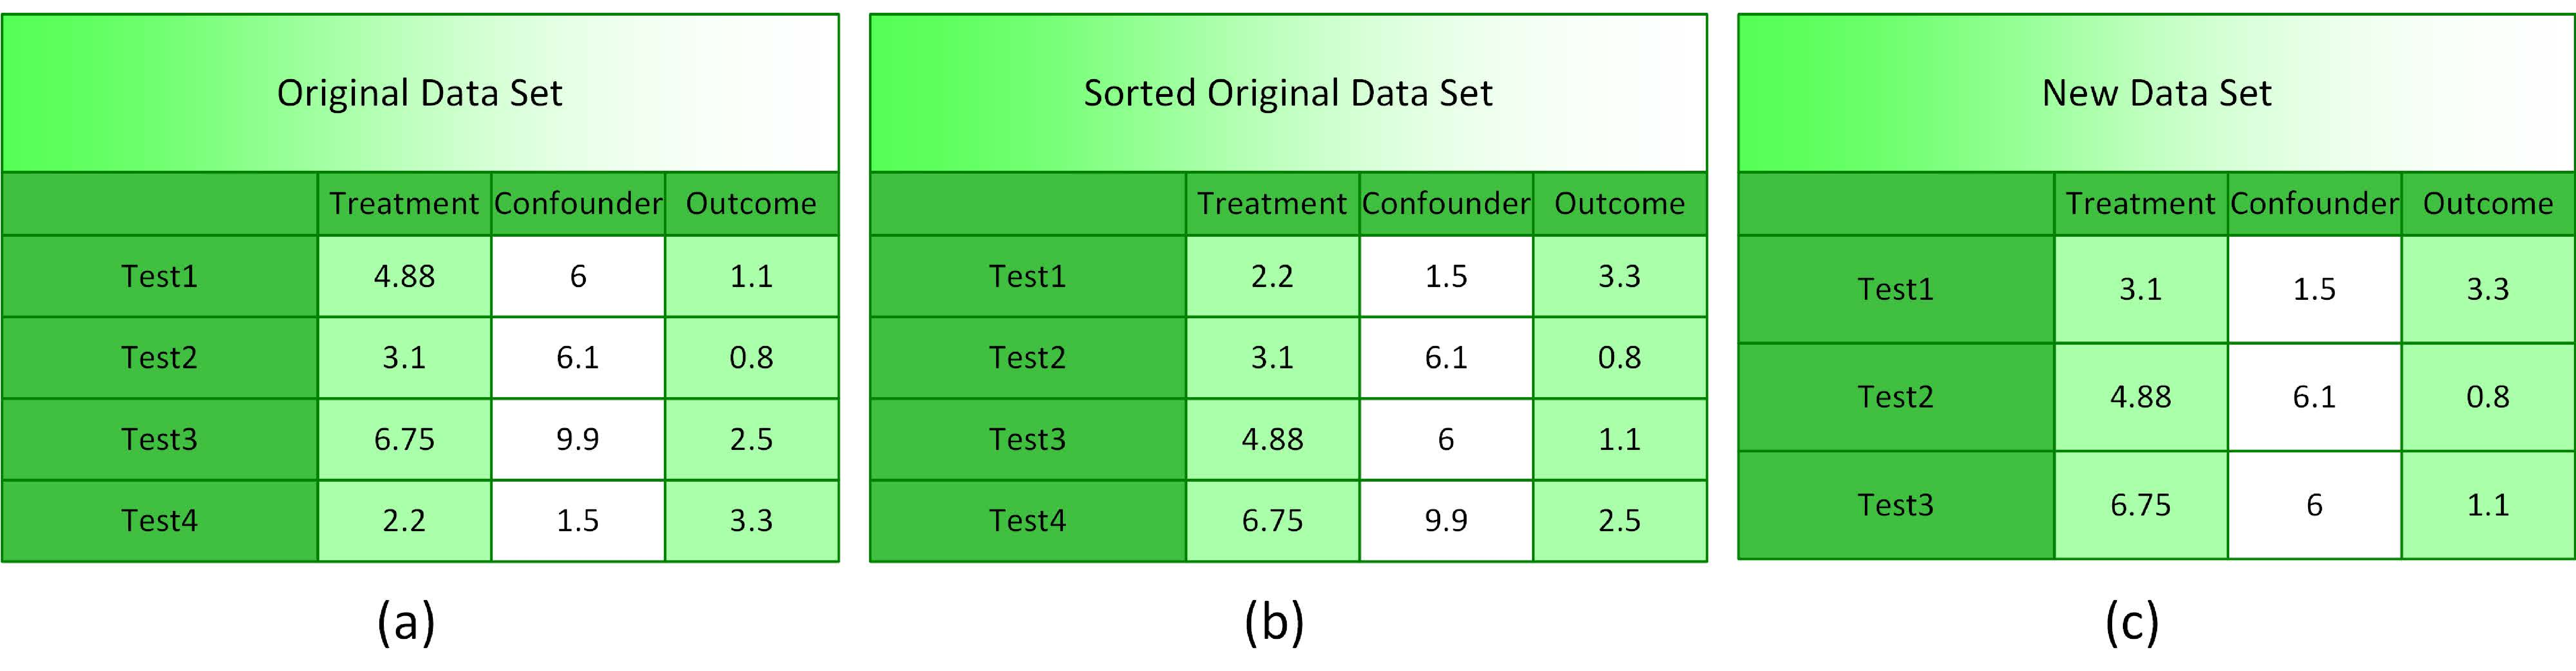
\includegraphics[width=1\textwidth]{chapter4_BART_ACE.pdf}
\caption{EXAMPLE OF TREATMENT VARIABLE INCREASE}
\label{bartace}
\end{figure*}

\section{EMPIRICAL EVALUATION}\label{BARTevaluation}% result

To evaluate the effectiveness of BART model, we conducted an empirical study on the same subject programs described in chapter 3.  The test suite is also identical to the test suite in section \ref{numfl_evaluation}.  Overall, there wre 92 faulty subject-programs versions with a single fault and 25 faulty subject-program versions with two faults. Ochiai, Dstar, SOBER, ESP-SIV and ESP-SCP were used as the base line techniques to be compared with BART model. We also compared the performance of the BART model with NUMFL-GPS and NUMFL-CBPS, which are described in chapter 3. We measured the costs of applying BART and the other metrics by the percentage of {\it subexpressions} that need to be examined, in decreasing order of suspiciousness scores, to find the fault, assuming the fault is recognized when it is encountered.

In the study, we used R package "BARTMachine" \cite{BARTMachine} to fit the BART model. We tried 10 trees and 50 trees in the sum-of-trees structure.  The BART model is fitted with both passing and failing tests. The number tests for each subject program ranged from 3000 to 8000 as shown in Table \ref{subpro}. To analyze the sensitivity of the BART model to the number of  tests, we also tried to train BART model with fewer data (300 tests). The sensitivity of the BART model to the number of trees and the number of tests are discussed in section \ref{BARTsensitivity}.

\subsection{Comparative Performance of BART vs. Baselines}

Figure \ref{BART_VS_Base} shows the results of comparisons of BART with each of the baseline metrics.  In each graph, the vertical axis represents the percentage improvement (reduction) in cost. The horizontal-axis represents different subject-program versions for which there are cost differences between the metrics, with each version represented by a vertical bar.   Bars above the zero-line represent versions for which BART performed better than the baseline metric and bars below zero represent versions for which BART performed worse.  The length of each bar represents the magnitude of the corresponding cost difference.

\textit{\textbf{ BART vs. Ochiai.}}  Over all 92 faulty subject-program versions, BART performed better than the Ochiai metric on 75 versions but BART performed worse on 17 versions.  There were 41 versions for which BART performed at least 20\% better than the Ochiai metric.  There were just 4 versions for which the latter performed better than BART.

\textit{\textbf{ BART vs. DStar.}}  BART performed better than DStar on 77 subject-program versions but BART performed worse than DStar on 15 versions.  BART performed at least 20\% better than DStar on 44 versions, whereas DStar performed at least 20\% better than BART on just 4 versions.

\textit{\textbf{ BART vs. ESP-SIV.}} BART performed better than ESP-SIV on 78 subject-program versions but BART performed worse than ESP-SIV on 14 versions.  BART performed at least 20\% better than ESP-SIV on 30 versions, whereas ESP-SIV never performed at least 20\% better than BART.

\textit{\textbf{ BART vs. ESP-SCP.}}  BART performed better than ESP-SCP on 75 subject-program versions but BART performed worse than ESP-SCP on 17 versions.  BART performed at least 20\% better than ESP-SIV on 22 versions, whereas ESP-SCP performed at least 20\% better than BART on just 2 versions.

\textit{\textbf{ BART vs. SOBER.}}  BART performed better than SOBER on 73 subject-program versions but BART performed worse than SOBER on 19 versions.  BART performed at least 20\% better than SOBER on 39 versions, whereas SOBER performed at least 20\% better than BART on just 5 versions.

\begin{sidewaysfigure}
\centering
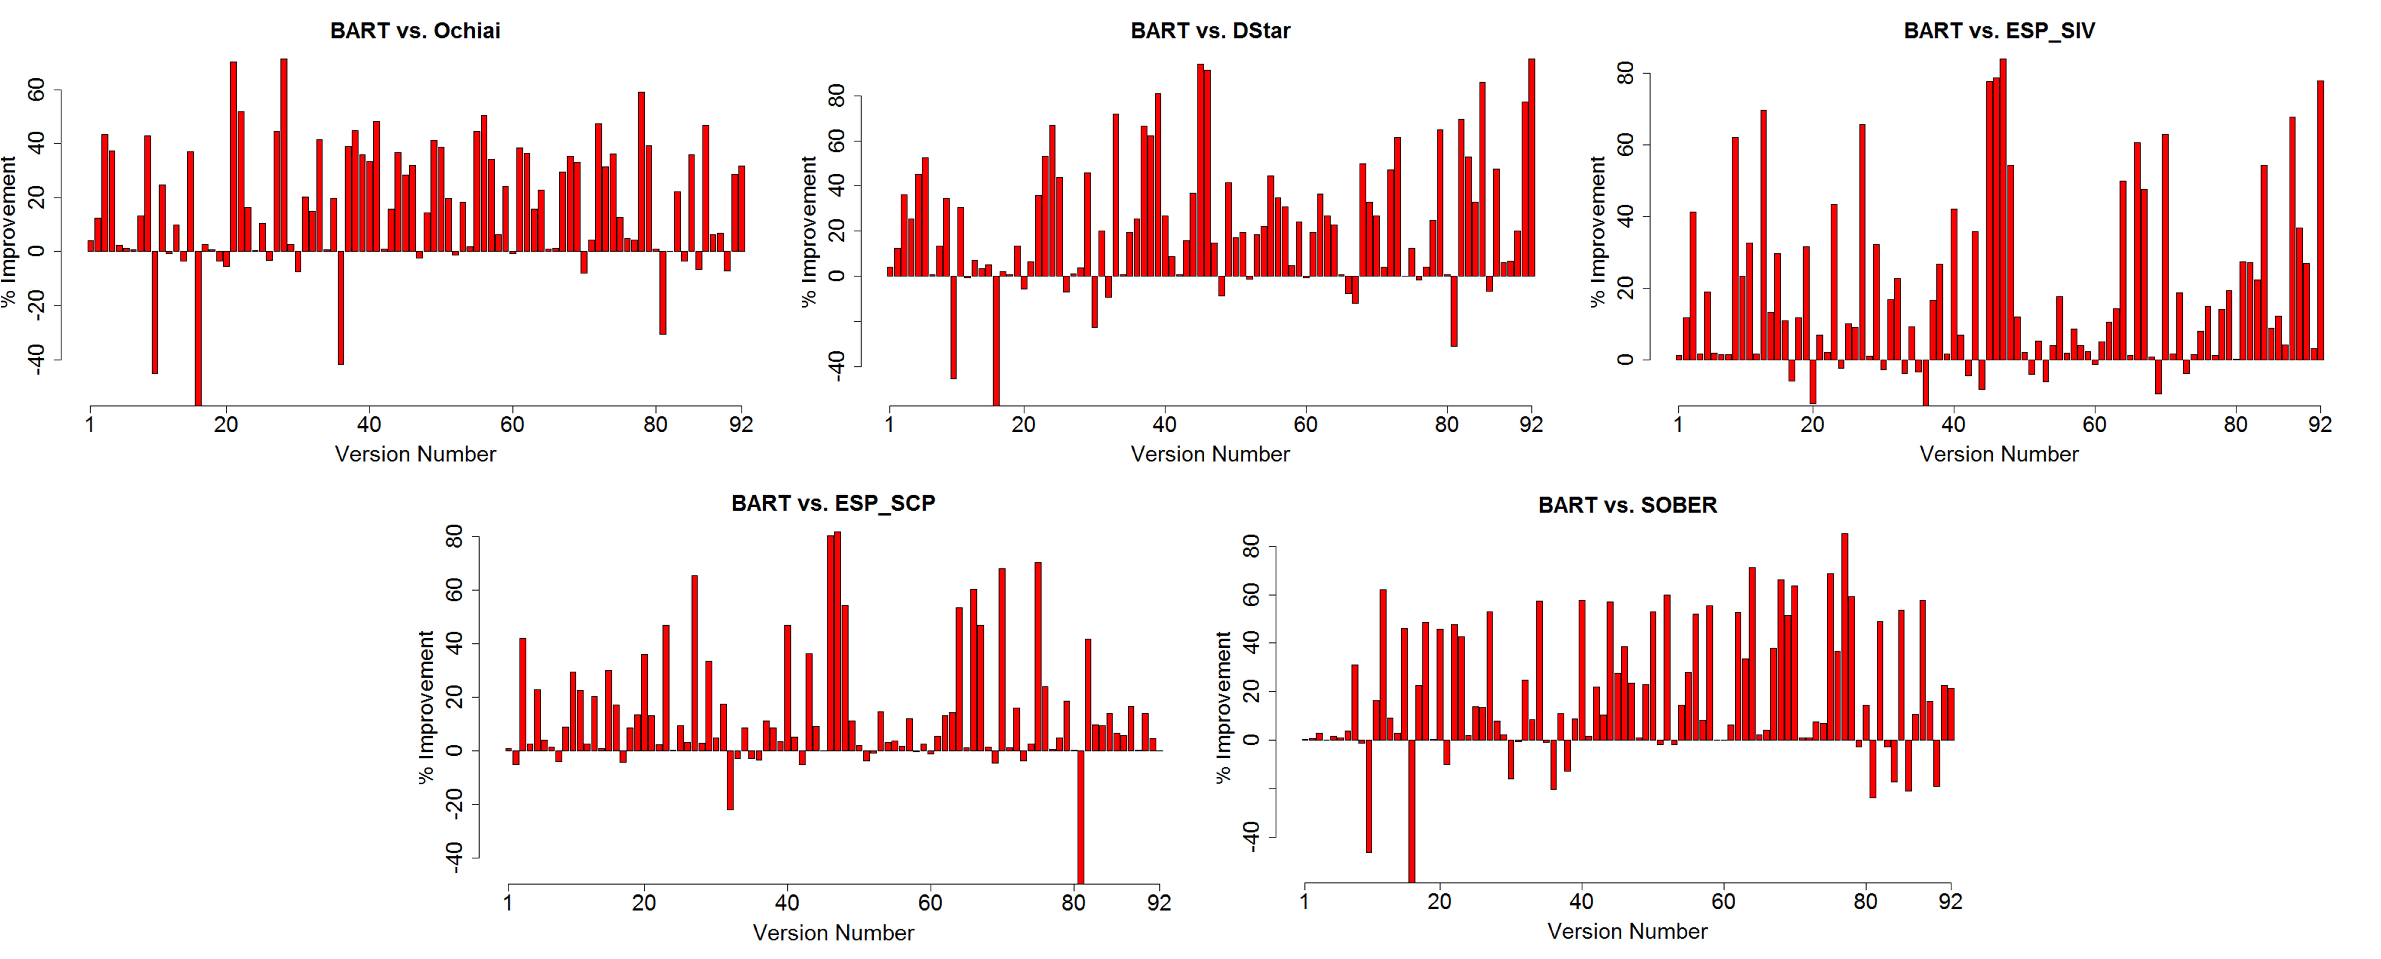
\includegraphics[width=\textwidth]{chapter4_BART_VS_Base.pdf}
\caption{Performance of BART relative to baseline metrics on individual single-fault program versions.}
\label{BART_VS_Base}
\end{sidewaysfigure}

Figure \ref{BART_VS_Base_M} contrasts the performance of BART on the individual two-fault program versions with that of the baseline metrics.  Over all 25 faulty subject-program versions, BART performed better than SOBER on 19 versions but performed worse on 6 versions.  There were 8 versions for which BART performed at least 10\% better than SOBER but 3 versions for which SOBER performed at least 10\% better than BART.  Ochiai performed better than BART on 5 versions but performed worse on 20 versions. BART performed at least 10\% better than Ochiai on 13 versions. BART performed better than both ESP-SIV and ESP-SCP on 20 versions.   BART performed better than DStar on 19 versions.

\begin{sidewaysfigure}
\centering
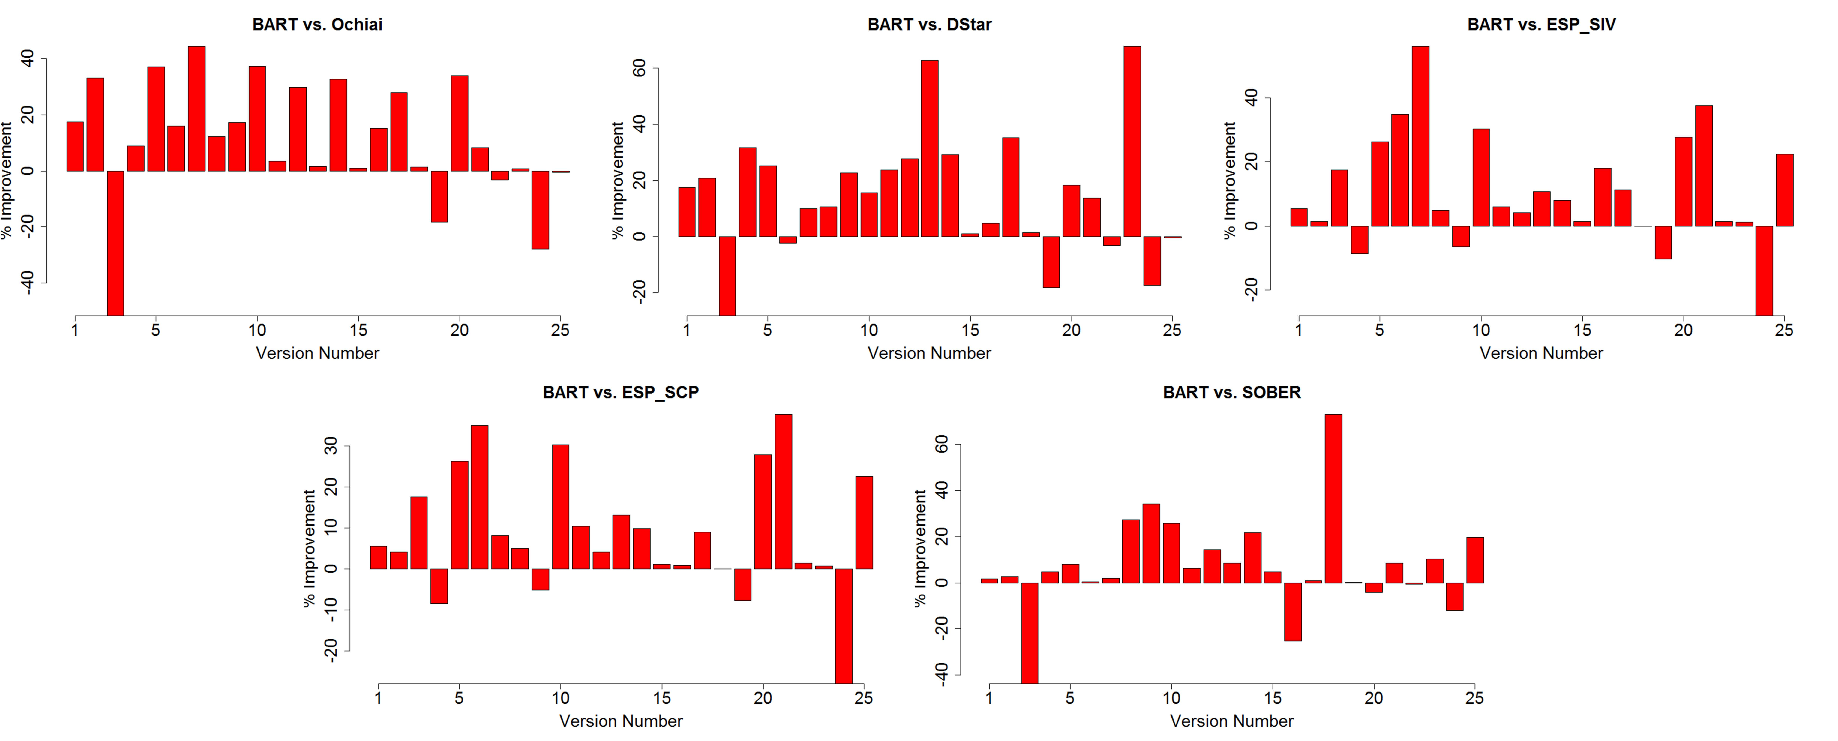
\includegraphics[width=\textwidth]{chapter4_BARTvsBase_M.pdf}
\caption{Performance of BART relative to baseline metrics on individual two-faults program versions.}
\label{BART_VS_Base_M}
\end{sidewaysfigure}


\subsection{BART Model vs NUMFL}
Table \ref{tableBARTvsNUMFL} shows the average percentage of subexpressions that had to be examined to find the fault, computed across all the faulty versions, for the BART model and NUMFL.  Because QRM is proved to have better performance than DLRM in chapter 3, here we only show the results of NUMFL-GPS-QRM and NUMFL-CBPS-QRM.  From Table \ref{tableBARTvsNUMFL}, there were 11 subject programs for which BART performed better than NUMFL-GPS-QRM. There were 5 subject programs for which NUMFL-GPS-QRM performed better than BART. BART performed better than NUMFL-CBPS-QRM on 14 subject programs. There were only 2 subject programs for which NUMFL-CBPS-QRM performed better than BART.

Figure \ref{BARTvsQRM} graphically contrasts the performance of BART and NUMFL-GPS-QRM on the single fault versions.  BART performed better than NUMFL-GPS-QRM on 54 versions, while NUMFL-GPS-QRM performed better on 38 versions.  BART performed at least 20\% better than NUMFL-GPS-QRM on 9 versions, whereas NUMFL-GPS-QRM performed at least 20\% better than BART on 6 versions. Figure \ref{BARTvsCBPS} graphically contrasts the performance of BART and NUMFL-CBPS-QRM on the single fault versions.  BART performed better than NUMFL-CBPS-QRM on 61 versions, while NUMFL-CBPS-QRM performed better on 31 versions.  BART performed at least 20\% better than NUMFL-CBPS-QRM on 17 versions, whereas NUMFL-CBPS-QRM performed at least 20\% better than BART on just 4 versions.

In summary, BART  performed better than both NUMFL-GPS-QRM and NUMFL-CBPS-QRM on single-fault programs. This suggests that BART model can well approximate the DRF of treatment variable and confounding variables.

\begin{table*}[htbp!]
\caption{AVERAGE FAULT LOCALIZATION COSTS OF BART AND NUMFL METRICS ON SINGLE-FAULT PROGRAM VERSIONS}
\label{tableBARTvsNUMFL}
\centering
      \begin{tabular}{|l|c|c|c|}
      \hline
\multirow{2}{*}{Subject Program}	& \multirow{2}{*}{BART}&	\multicolumn{2}{|c|}{{\bf NUMFL}}	\\	\cline{3-4}
& & GPS-QRM	&CBPS-QRM \\ \hline
Apache\_EigenDecompose &	2.50\%&	12.3\%	&	8.8\%	\\	\hline
Apache\_DScompiler&	9.72\%&	11\%	&	12\%	\\	\hline
Apache\_BigMatrix	&	9.00\%&11.4\%	&	9.9\%	\\	\hline
Apache\_Rotation3D&	9.07\%&	8\%	&	18.9\%	\\	\hline
Ojaljo\_SchurDecompose&	10.61\%&	11.4\%	&	14\%	\\	\hline
Jama\_MatrixDecompose	&11.62\%&	14.2\%	&	23\%	\\	\hline
SciMark\_LU&8.33	\%&	15.3\%	&	27.8\%	\\	\hline
SciMart\_FFT&	 27.59\%&	9.5\%	&	19.8\%	\\	\hline
Apache\_SymmLQ&	 1.75\%&	2.6\%	&	4.4\%	\\	\hline
Apache\_SplineInterpolator&	 37.78\%&	31.7\%	&	35\%	\\	\hline
Apche\_SimpleRegress&	 1.70\%&	4.3\%	&	17\%	\\	\hline
Apache\_SchurTransformer&	 4.56\%&	3.3\%	&	14.9\%	\\	\hline
Apache\_MillerUpdatRegress&	 1.24\%&	7.5\%	&	9.9\%	\\	\hline
Apache\_HarmonicFitter&	30.10\%&	27.3\%	&	32\%	\\	\hline
Apache\_FastSine&	1.53\%&	1.5\%	&	13\%	\\	\hline
Apache\_FastCosine	&1.29	\%&1.3\%	&	1.2\%	\\	\hline
Average Cost	&	10.52\%&10.8\%	&	16.4\%	\\	\hline
\end{tabular}
\end{table*}

\begin{figure*}[!thpb]
\centering
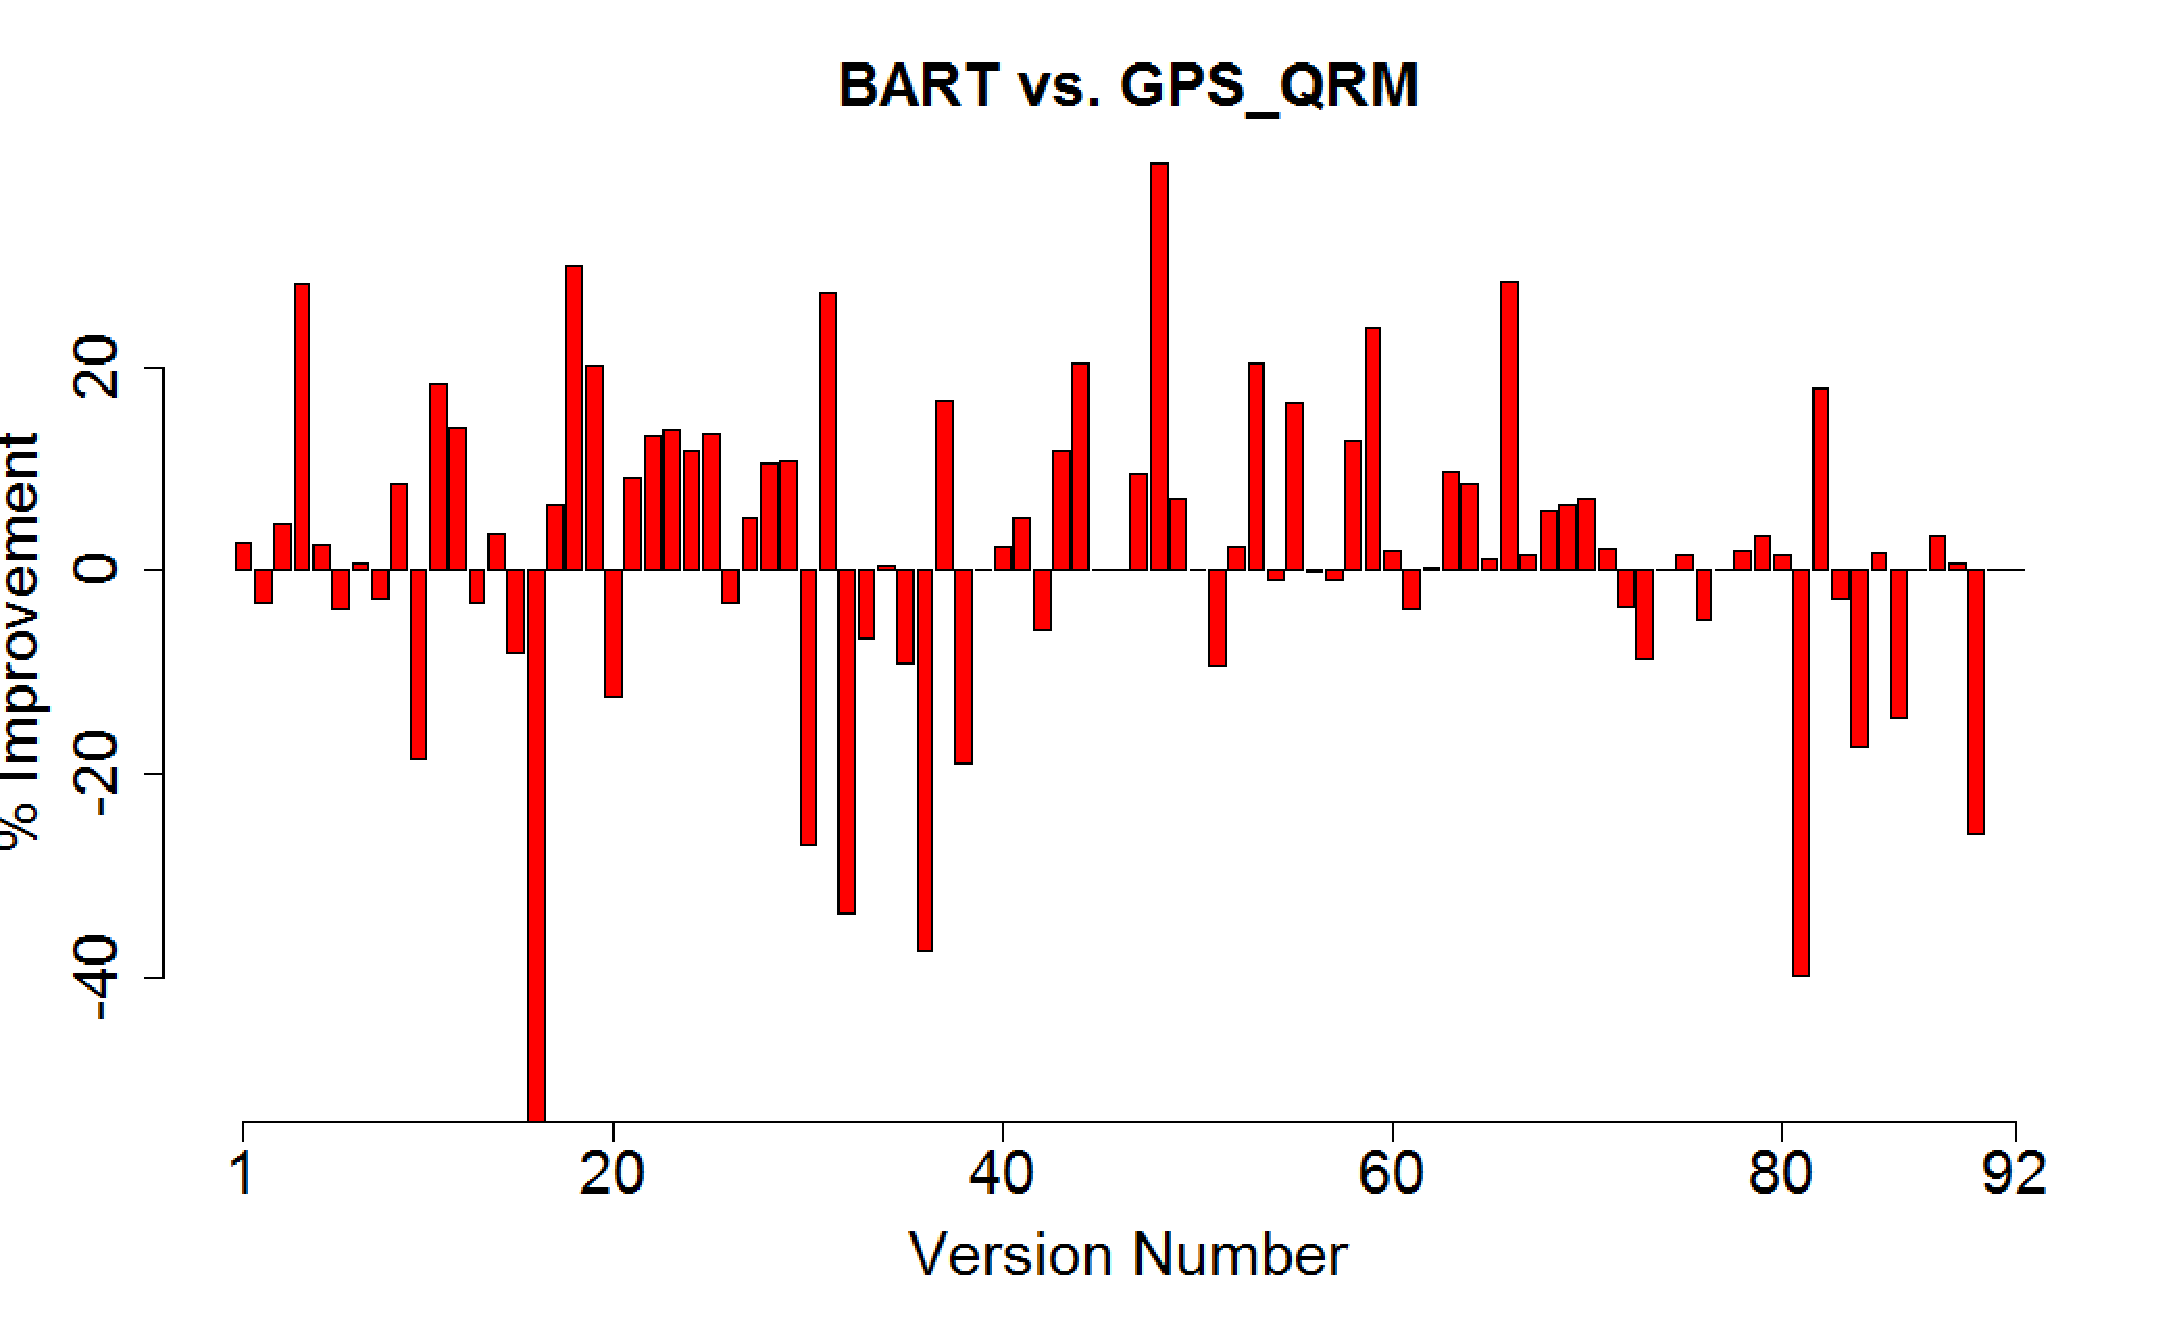
\includegraphics[width=0.8\textwidth]{chapter4_BARTvsGPS_QRM.pdf}
\caption{Relative performance of BART and NUMFL-GPS-QRM on individual single-fault program versions.}
\label{BARTvsQRM}
\end{figure*}

\begin{figure*}[!thpb]
\centering
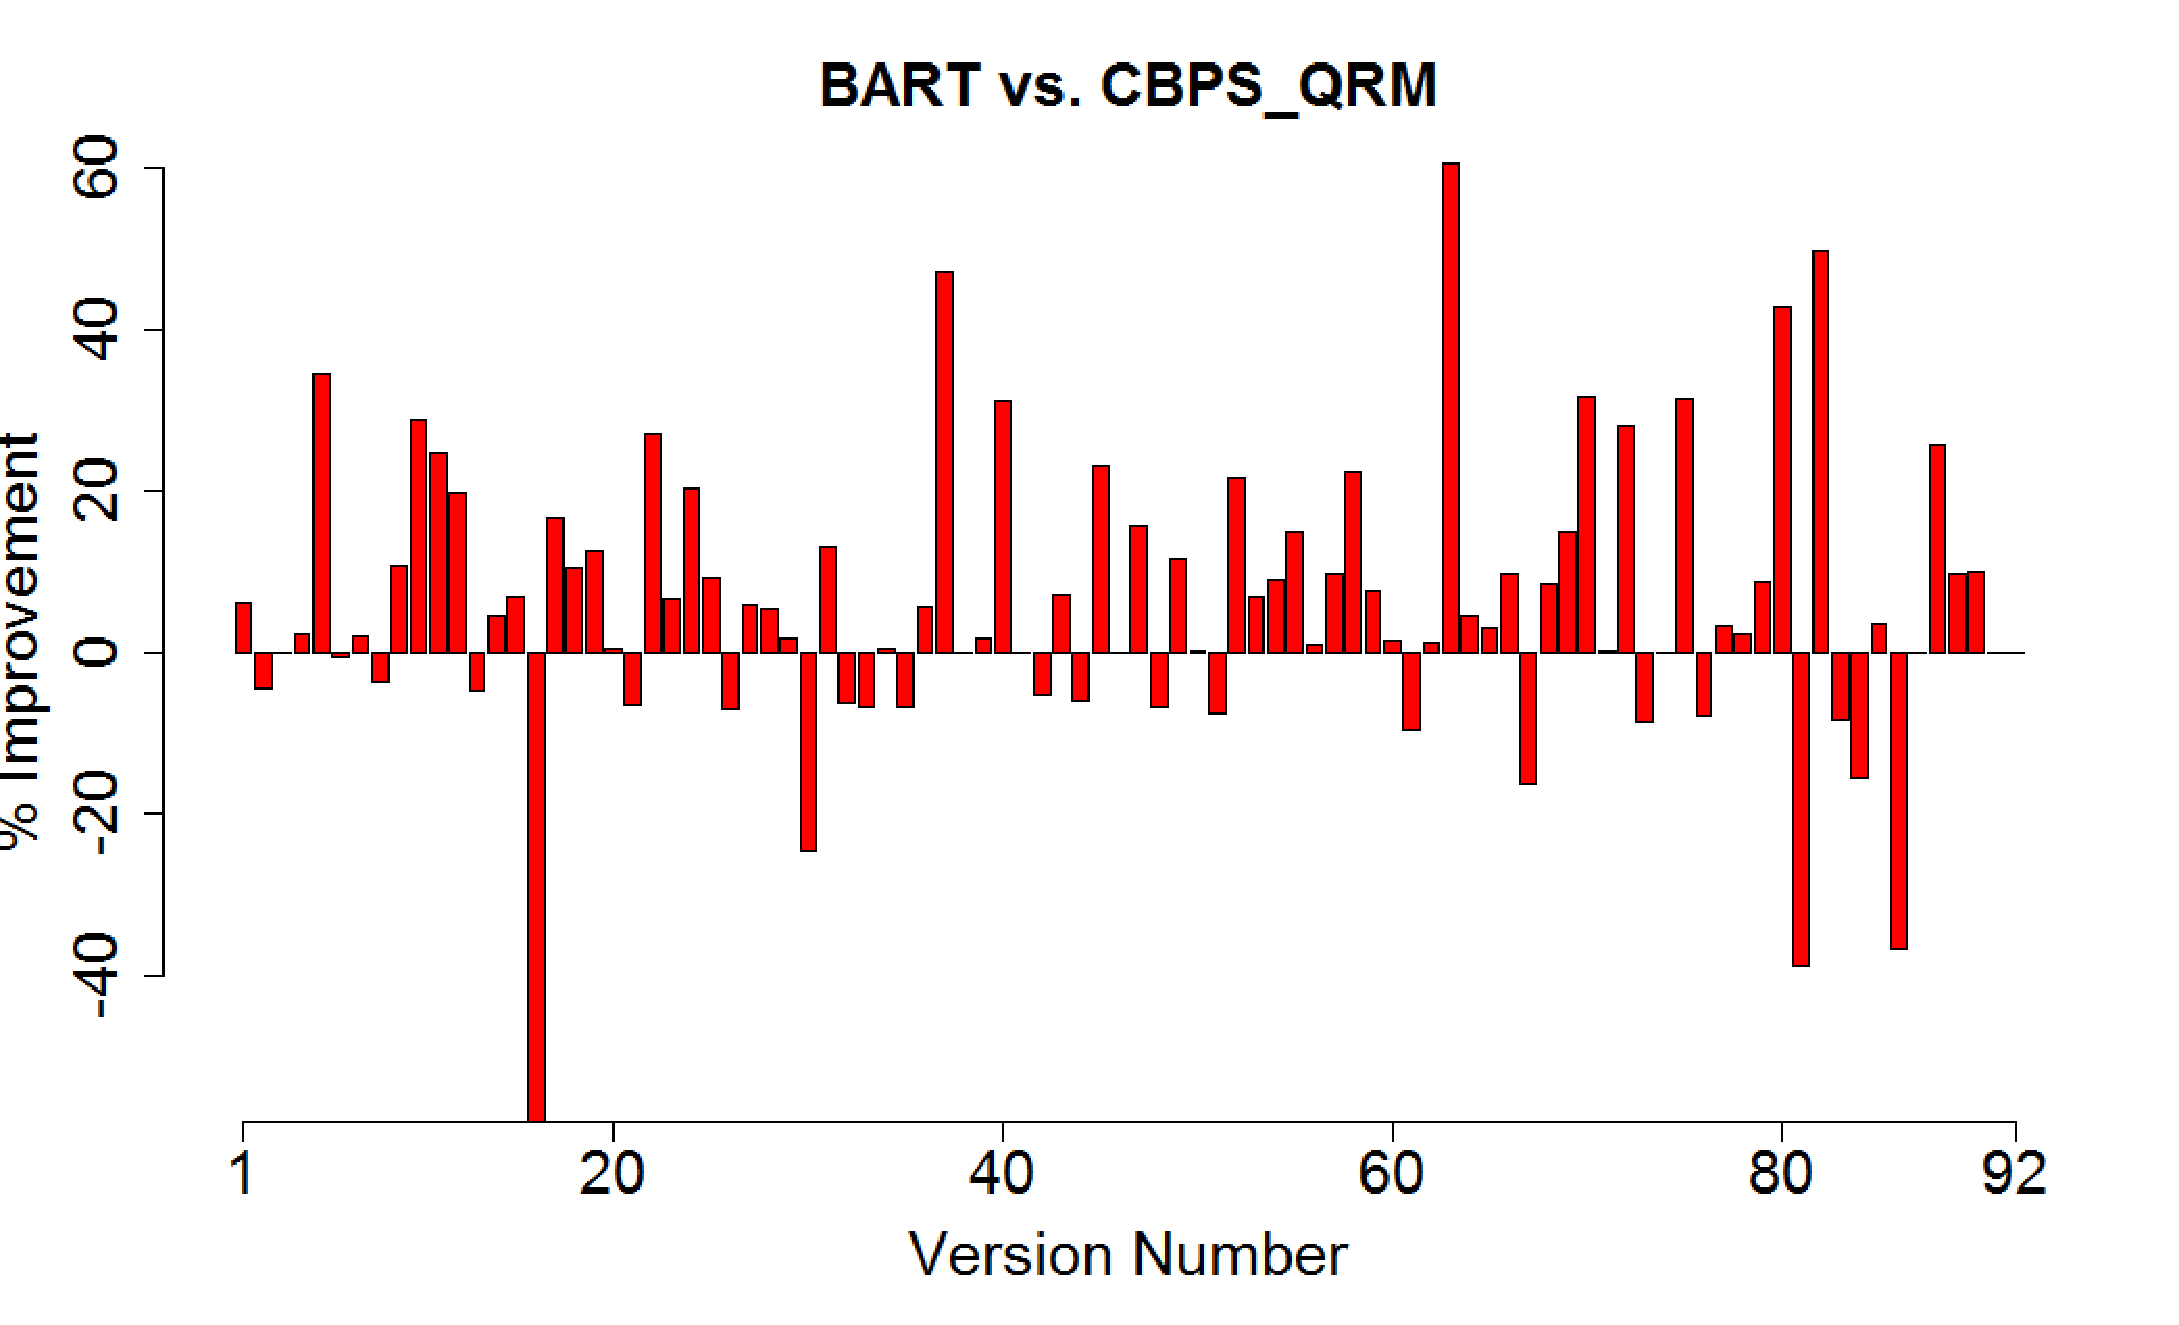
\includegraphics[width=0.8\textwidth]{chapter4_BARTvsCBPS.pdf}
\caption{Relative performance of NUMFL-CBPS-QRM on individual single-fault program versions.}
\label{BARTvsCBPS}
\end{figure*}

Table \ref{tableBARTvsNUMFL_M} shows the average cost, over the faulty versions of each subject program into which two-fault were injected, of localizing the first fault to be found, for both BART and NUMFL.  From Table \ref{tableBARTvsNUMFL_M}, BART and NUMFL-GPS-QRM have similar performance on two faults subject programs. BART performed better than NUMFL-GPS-QRM on the versions of  2 subject programs, but performed worse than NUMFL-GPS-QRM on the versions of 3 subject program.  BART performed better than NUMFL-CBPS-QRM on the versions of 4 subject programs, but performed worse than NUMFL-CBPS-QRM on the versions of only 1 subject program.

Figure \ref{BARTvsGPS_M} graphically contrasts the performance of the BART and NUMFL-GPS-QRM on the individual two-fault versions.  BART performed better than NUMFL-GPS-QRM on 13 versions and BART performed worse on 12 versions.  BART performed at least 10\% better than NUMFL-GPS-QRM on 7 versions, whereas NUMFL-GPS-QRM performed at least 10\% better than BART on just 1 version. Figure \ref{BARTvsCBPS_M} graphically contrasts the performance of the BART and NUMFL-CBPS-QRM on the individual two-fault versions.  BART performed better than NUMFL-CBPS-QRM on 13 versions and BART performed worse on 12 versions.  BART performed at least 10\% better than NUMFL-CBPS-QRM on 7 versions, whereas NUMFL-CBPS-QRM performed at least 10\% better than BART on just 1 version.

\begin{table*}[htbp!]
\caption{AVERAGE FAULT LOCALIZATION COSTS OF BART AND NUMFL ON TWO-FAULT PROGRAM VERSIONS}
\label{tableBARTvsNUMFL_M}
\centering
      \begin{tabular}{|l|c|c|c|}
      \hline
\multirow{2}{*}{Subject Program}	& \multirow{2}{*}{BART}&	\multicolumn{2}{|c|}{{\bf NUMFL}}	\\	\cline{3-4}
& & GPS-QRM	&CBPS-QRM \\ \hline
Apache\_EigenDecompose	&7.98	\%&10.3\%	&	11.1\%	\\	\hline
Apache\_DScompiler	&	5.13\%&4.5\%	&	5.9\%	\\	\hline
Apache\_Rotation3D	&	10.69\%&7.0\%	&	3.0\%	\\	\hline
Ojaljo\_SchurDecompose	&17.55	\%&5.4\%	&	19.8\%	\\	\hline
Jama\_MatrixDecompose	&	4.65\%&14.1\%	&	23.4\%	\\	\hline
{\bf Average Cost} &9.20\% &8.26\% &12.64\%\\ \hline
\end{tabular}
\end{table*}

\begin{figure*}[!thpb]
\centering
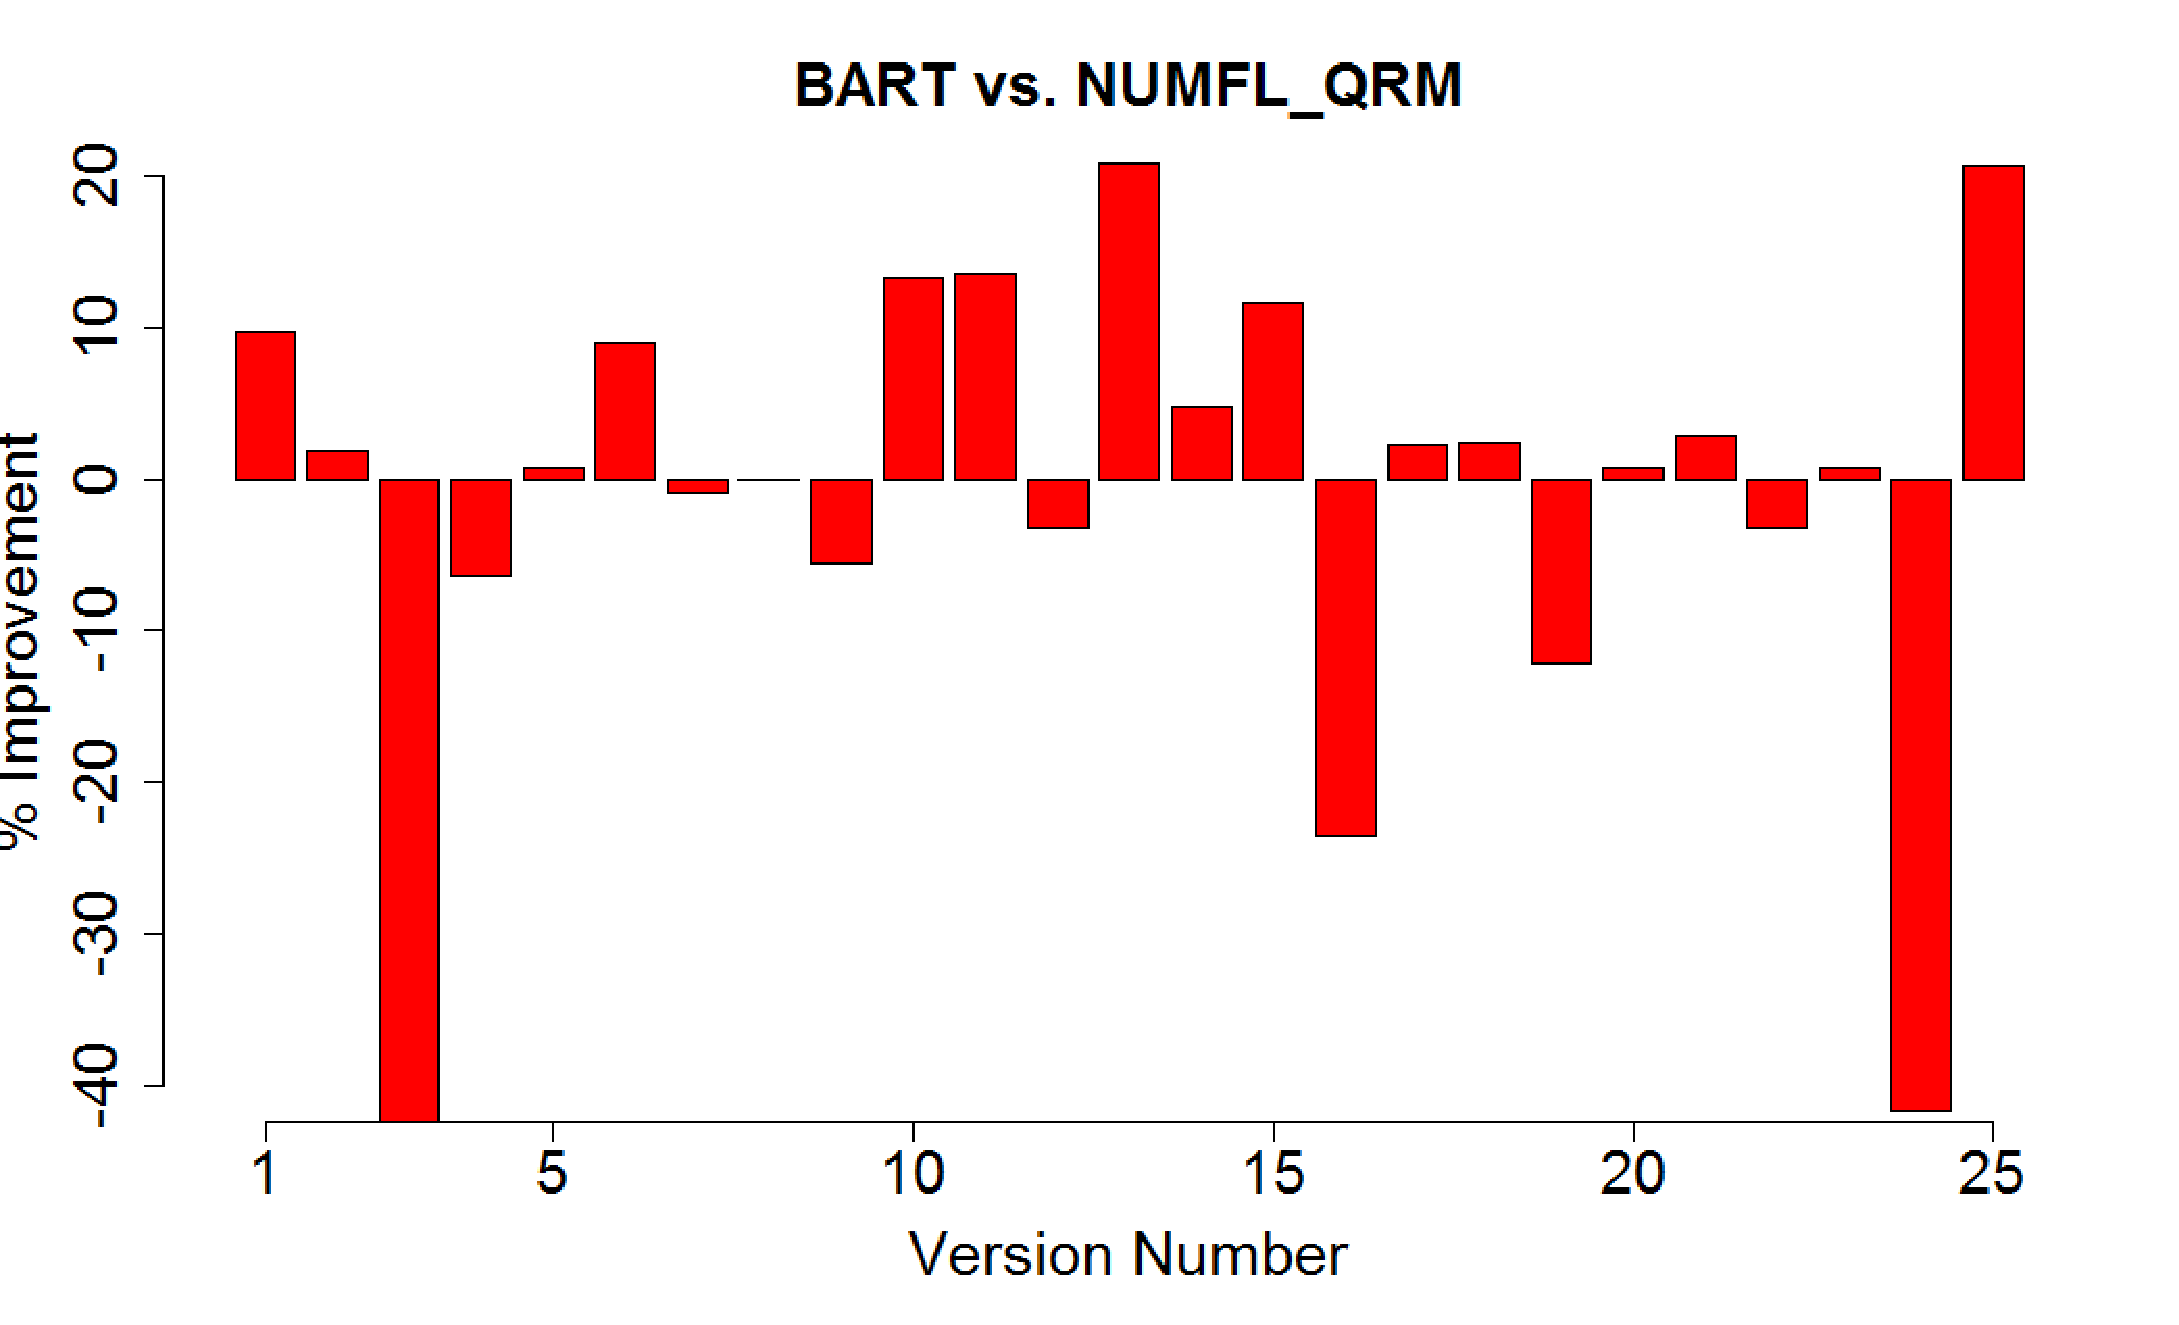
\includegraphics[width=0.8\textwidth]{chapter4_BARTvsGPS_QRM_M.pdf}
\caption{Relative performance of BART and NUMFL-GPS-QRM on two-fault program versions.}
\label{BARTvsGPS_M}
\end{figure*}

\begin{figure*}[!thpb]
\centering
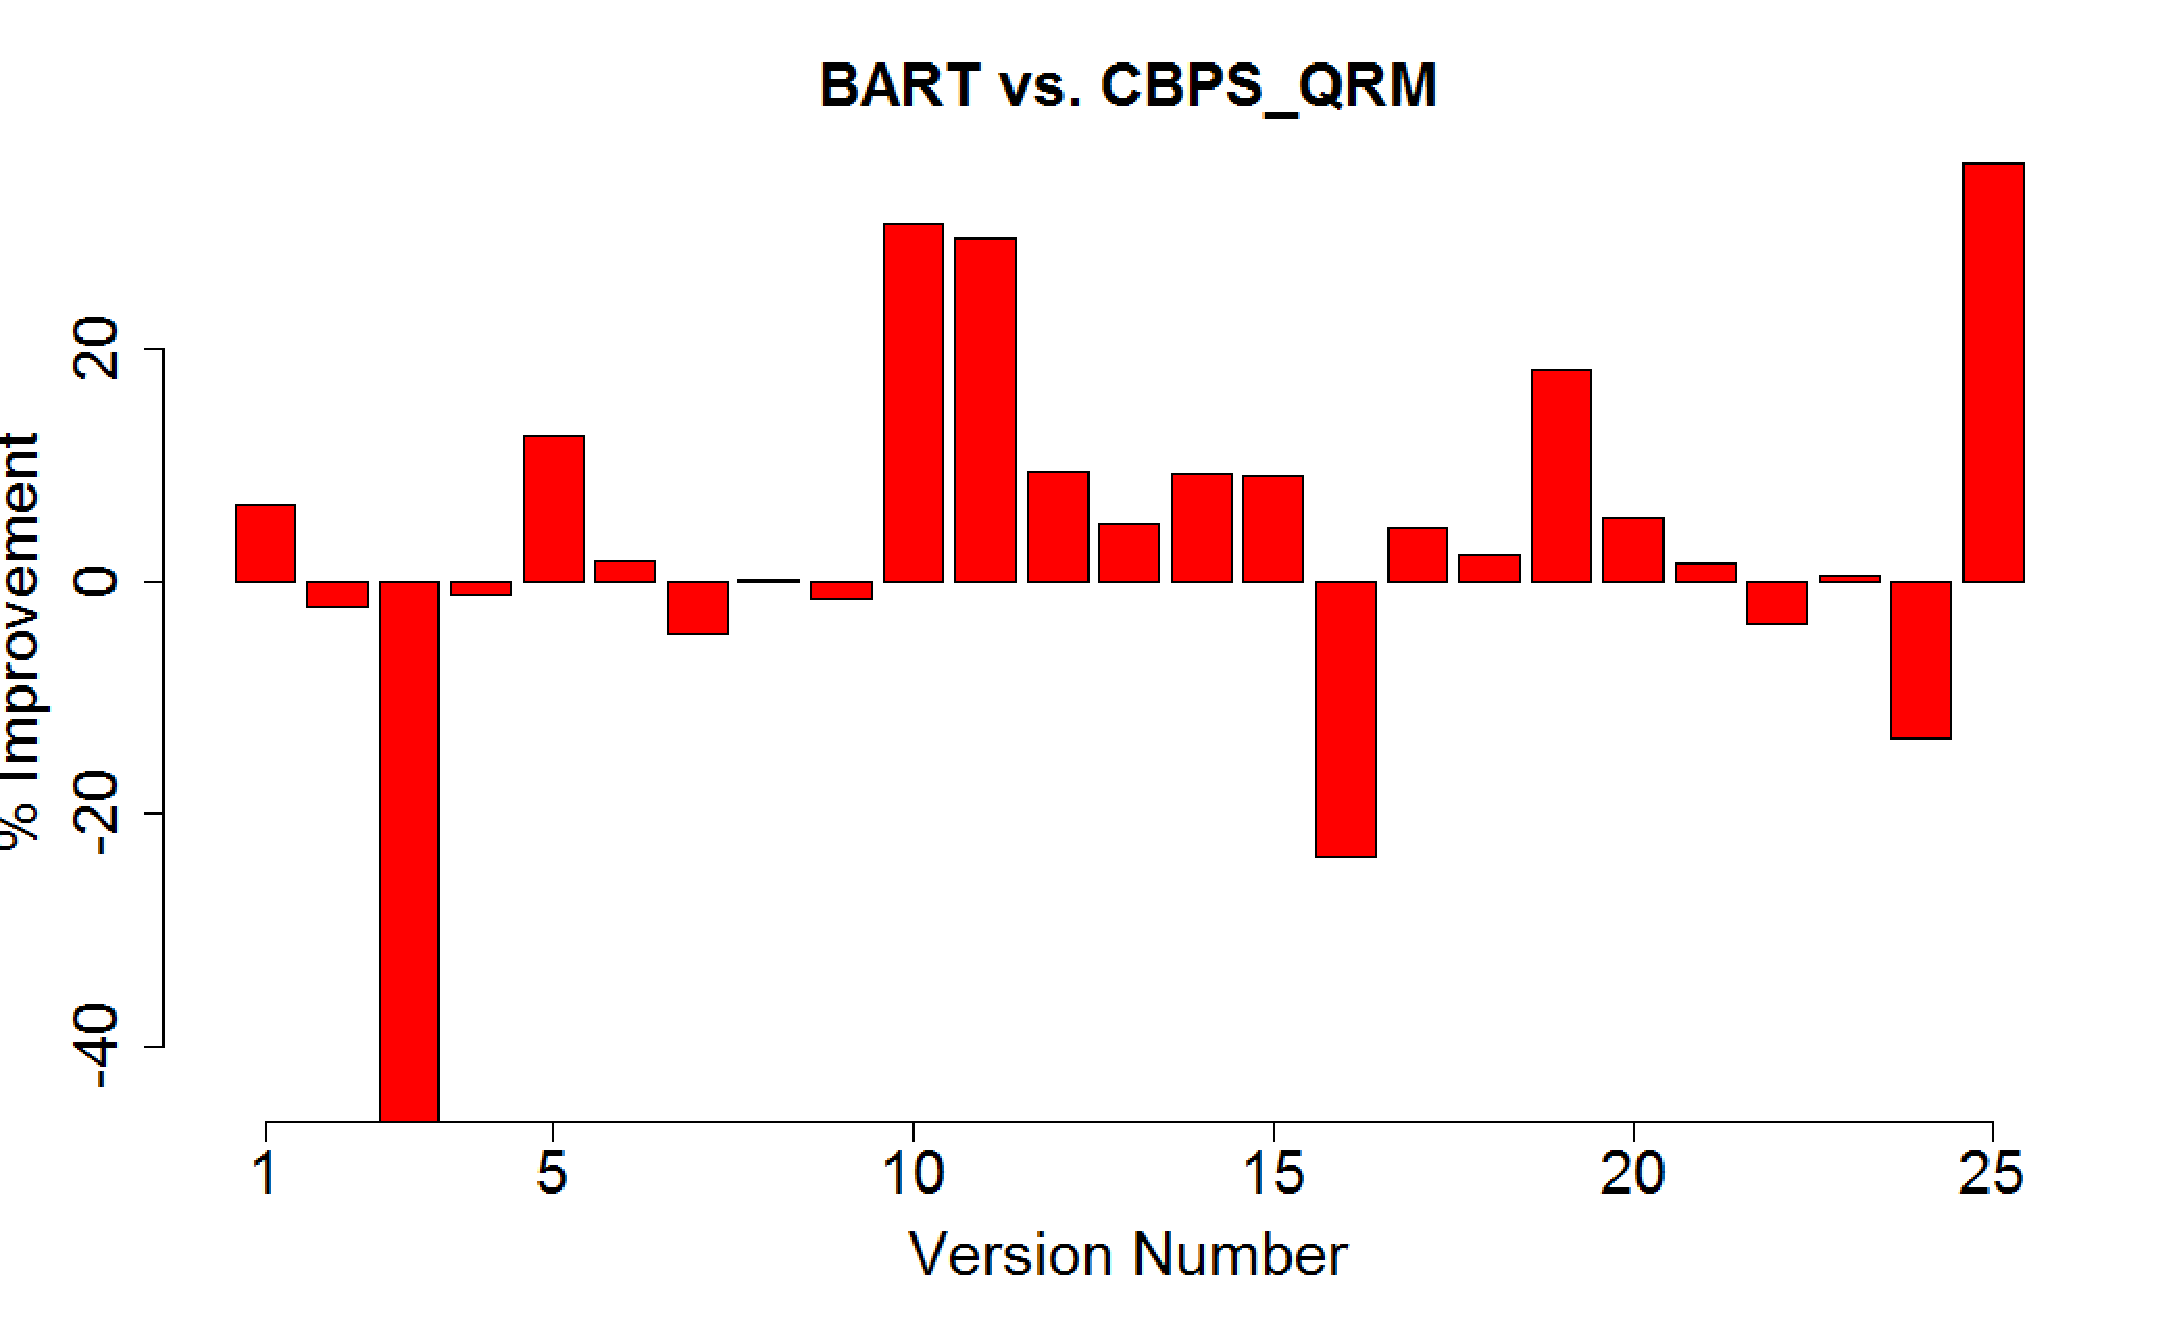
\includegraphics[width=0.8\textwidth]{chapter4_BARTvsCBPS_M.pdf}
\caption{Relative performance of BART and NUMFL-CBPS-QRM on two-fault program versions..}
\label{BARTvsCBPS_M}
\end{figure*}

\subsection{Sensitivity of BART model on the number of trees and  the number of tests}\label{BARTsensitivity}

In previous sections, we used the data from all tests to fit a BART model with 10 trees in the sum-of-trees structure. In this section, we examine whether if increasing number of trees or decreasing the number of tests would influence the performance of BART. In Table \ref{sensitivity}, the first column is the fault localization cost of the BART model containing 10 trees, and fitted with 3000 tests. The second column is the fault localization cost of the BART model containing 50 trees, and fitted with 3000 tests. The third column is the fault localization cost of the BART model containing 10 trees, but fitted with only 300 tests. From Table \ref{sensitivity}, it can be seen that when we increased the number of trees from 10 to 50, the BART model has better performance on 6 subject programs. But there are also 6 subject program where the BART model's performance became worse after the number of trees was increased. The average cost across 16 subject programs is roughly same: 10.52\% for the BART model with 10 trees and 10.58\% for the BART model with 50 trees. This suggests that 10 trees are enough to handle the nonlinearity problem in AFCE estimation at least with programs that are similar to those used in the study.  When we decrease the number of tests to 300, the average cost is slightly increased to 10.74\%.  This means that the BART model does not require a large number of tests to localize faults in numerical softwares.

\begin{table*}[htbp!]
\caption{AVERAGE FAULT LOCALIZATION COSTS OF BART MODEL WITH DIFFERENT NUMBER OF TREES AND DIFFERENT NUMBER OF TESTS ON SINGLE-FAULT PROGRAM VERSIONS }
\label{sensitivity}
\centering
      \begin{tabular}{|l|c|c|c|}
      \hline
\multirow{2}{*}{{\bf Subject Program}}	&	\multicolumn{3}{|c|}{{\bf BART Model}}	\\	\cline{2-4}
& 10 trees & 50 trees & 300 tests\\ \hline
Apache\_EigenDecompose			&	2.50	\%	&	3.07	\%	&	2.38	\%	\\ \hline
Apache\_DScompiler			&	9.72	\%	&	8.61	\%	&	9.64	\%	\\ \hline
Apache\_BigMatrix			&	9.00	\%	&	9.05	\%	&	9.00	\%	\\ \hline
Apache\_Rotation3D			&	9.07	\%	&	8.73	\%	&	8.16	\%	\\ \hline
Ojaljo\_SchurDecompose			&	10.61	\%	&	9.89	\%	&	11.44	\%	\\ \hline
Jama\_MatrixDecompose			&	11.62	\%	&	11.16	\%	&	11.32	\%	\\ \hline
SciMark\_LU			&	8.33 \%	&	9.72	\%	&	6.94	\%	\\ \hline
SciMart\_FFT			&	27.59	\%	&	26.72	\%	&	27.59	\%	\\ \hline
Apache\_SymmLQ			&	1.75	\%	&	1.75	\%	&	1.75	\%	\\ \hline
Apache\_SplineInterpolator			&	37.78	\%	&	40	\%	&	45.56	\%	\\ \hline
Apche\_SimpleRegress			&	1.70	\%	&	1.70	\%	&	1.70	\%	\\ \hline
Apache\_SchurTransformer			&	4.56	\%	&	4.88	\%	&	4.23	\%	\\ \hline
Apache\_MillerUpdatRegress			&	1.24	\%	&	1.24	\%	&	1.24	\%	\\ \hline
Apache\_HarmonicFitter			&	30.10	\%	&	30.08	\%	&	28.06	\%	\\ \hline
Apache\_FastSine			&	1.53	\%	&	1.53	\%	&	1.53	\%	\\ \hline
Apache\_FastCosine			&	1.29	\%	&	1.29	\%	&	1.29	\%	\\ \hline
Average Cost 	&	10.52\% 	&10.58\% 	&10.74\%	\\ \hline
\end{tabular}
\end{table*}

\subsection{Computation Time Analysis}
In this study, we used a Dell Precision T5600 with two 2.30 GHz Intel Xeon CPUs and 64 GB RAM. Table \ref{BARTcomputetime} summarized the average computation time of the three BART models described in last section on each subject program.  When the number of trees increased from 10 to 50, the average computation cost nearly doubled. If we reduced number the tests from more than 3000 to 300, the computation cost was reduced more than 50\%.  From Table \ref{BARTcomputetime} and Table \ref{sensitivity}, we can conclude that the BART model with 10 trees and fitted with 300 tests had the best cost-performance ratio among the three BART models fitted with different settings. But we also need to point out that even when the BART model is fitted with 300 tests, its computation cost is still about twice of the computation cost of NUMFL. Thus, computation cost is a weakness of applying BART on localizing faults in numerical softwares. 

\begin{table*}[htbp!]
\caption{AVERAGE COMPUTATION TIME OF BART ON SINGLE-FAULT PROGRAM VERSIONS }
\label{BARTcomputetime}
\centering
      \begin{tabular}{|l|c|c|c|}
      \hline
\multirow{2}{*}{{\bf Subject Program}}	&	\multicolumn{3}{|c|}{Average Computation Time (Secs)}	\\	\cline{2-4}
& 10 trees & 50 trees & 300 tests\\ \hline

Apache\_EigenDecompose	&	2856.73	&	5530.20	&	1205.97	\\ \hline
Apache\_DScompiler	&	628.31	&	1243.78	&	274.88	\\ \hline
Apache\_BigMatrix	&	696.58	&	1337.73	&	292.28	\\ \hline
Apache\_Rotation3D	&	2668.41	&	5550.45	&	1082.64	\\ \hline
Ojaljo\_SchurDecompose	&	2636.96	&	5013.37	&	1313.53	\\ \hline
Jama\_MatrixDecompose	&	3134.49	&	6005.71	&	1262.88	\\ \hline
SciMark\_LU	&	167.94	&	332.45	&	121.38	\\ \hline
SciMart\_FFT	&	393.26	&	842.31	&	234.09	\\ \hline
Apache\_SymmLQ	&	908.12	&	1986.32	&	245.21	\\ \hline
Apache\_SplineInterpolator	&	364.80	&	747.42	&	135.00	\\ \hline
Apche\_SimpleRegress	&	823.34	&	1685.88	&	227.27	\\ \hline
Apache\_SchurTransformer	&	768.44	&	1539.44	&	315.65	\\ \hline
Apache\_MillerUpdatRegress	&	396.10	&	808.59	&	198.61	\\ \hline
Apache\_HarmonicFitter	&	326.09	&	673.73	&	120.28	\\ \hline
Apache\_FastSine	&	1006.86	&	2064.98	&	259.78	\\ \hline
Apache\_FastCosine	&	1089.13	&	2229.39	&	294.56	\\ \hline
\end{tabular}
\end{table*}

\section{RELATED WORK}\label{BARTrelatedwork}
The most related works to this study are those using BART model to estimate treatment causal effect. Hill et al. proposed to apply BART model for causal inference and data science \cite{hill2012bayesian, hill2013assessing}. In the paper, they designed the method of using BART to estimate average causal effect of binary treatment variable and discussed how to use BART to handle continuous treatment variables and outcome missing data. Later, Green et al. applied BART to model heterogeneous treatment effects \cite{green2012modeling}. Sparapani et al. extends the usefulness of BART in medical applications by addressing needs arising in survival analysis \cite{sparapani2016nonparametric}.

Another related work is using tree structure in fault localization. Chen et al \cite{chen2004failure} present a decision tree learning approach to identify the causes of failures in internet sites. Francis et al \cite{francis2004tree} use tree based method to classify software failures. Kiciman et al \cite{kiciman2005root} use decision tree to diagnose which component of large scale systems is the root cause of failure. However, unlike our models, all their works do not localize the fault on statement level.

\section{CONCLUSION}\label{BARTconclusion}
The BART model is a Bayesian non-parametric model which can capture both nonlinearities and interactions between variables without knowing how these variables are parametrically related . BART uses a sum of trees structure to approximate the dose-response function of continuous treatment variables. The AFCE can be estimated by averaging the predicted causal effect of treatment on the outcome at each observation unit. We reported the result of an empirical comparison of BART model with several competing fault localization metrics on both single-fault subject programs and multiple-fault subject programs. The BART model performed significantly better than the other techniques. We also compare the BART model with NUMFL, which was introduced in chapter 3. The result shows BART model outperformed NUMFL on single-fault programs. With multiple-fault programs, BART and NUMFL had similar performances.  We also study the sensitivity of the BART model to the number of trees and the number of tests. The results show BART is robust on the sample size and number of trees.   